\chapter{Background}\label{chap:background}

\section{Definition of terms}
\subsection{Scholarly discourse}

\section{Theoretical background}
\subsection{Supervised machine learning}

explain all the things.

definition of terms (claim, etc.), mby also distinction of integral/non-integral and syntactic/non-syntactic citations here?

supervized ml (briefly)
% michael:
% - peculiarities of CiteRec (many papers, few users, even in the field of rec systems);
% - diverse nature of publications to be parsed (what data can be extracted from papers, ...);
% in general: Only focus on really, i.e., directly relevant items/concepts mentioned later in the thesis.

global/local citation (for local especially explain harvesting citation contexts and comparing aggregrates to input)

citation marker

four types of numbers (citing/cited documents, reference items citation context)

reference resolution

\begin{figure}
  \centering
    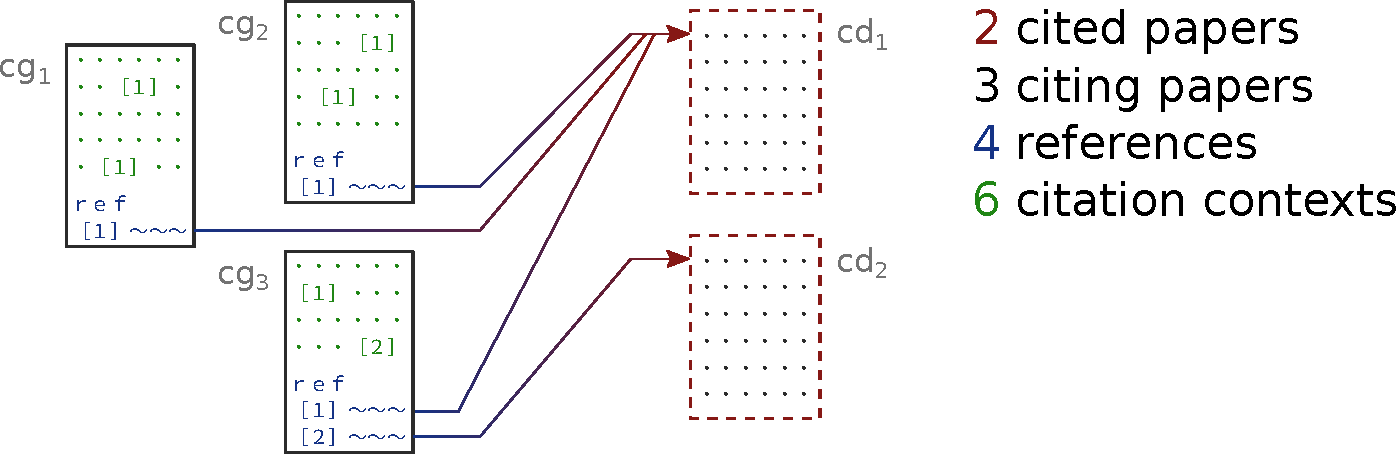
\includegraphics[width=\textwidth]{figures/background/four_types_of_numbers_vertsqueeze.pdf}
  \caption[Four types of numbers.]{Four types of numbers. A toy example with citation pairs $cg_1\rightarrow cd_1$, $cg_2\rightarrow cd_1$, $cg_3\rightarrow cd_1$, $cg_3\rightarrow cd_2$ resulting in 2 cited papers, 3 citing papers, 4 references and 6 citation contexts.}
  \label{fig:fournumbers}
\end{figure}
